\documentclass{beamer}

\mode<presentation>
\usepackage{amsmath,amssymb,mathtools}
\usepackage{textcomp}
\usepackage{gensymb}
\usepackage{adjustbox}
\usepackage{subcaption}
\usepackage{enumitem}
\usepackage[utf8]{inputenc}
\usepackage{amssymb}
\usepackage{enumitem}
\setlist{nosep} % optional: removes vertical gaps
\setlist[enumerate]{label=\arabic*)} % custom numbering if you want

\usepackage{multicol}
\usepackage{listings}
\usepackage{url}
\usepackage{graphicx} % <-- needed for images
\def\UrlBreaks{\do\/\do-}

\usetheme{Boadilla}
\usecolortheme{lily}
\setbeamertemplate{footline}{
  \leavevmode%
  \hbox{%
  \begin{beamercolorbox}[wd=\paperwidth,ht=2ex,dp=1ex,right]{author in head/foot}%
    \insertframenumber{} / \inserttotalframenumber\hspace*{2ex}
  \end{beamercolorbox}}%
  \vskip0pt%
}
\setbeamertemplate{navigation symbols}{}

\lstset{
  frame=single,
  breaklines=true,
  columns=fullflexible,
  basicstyle=\ttfamily\small % Adjusted for better readability
}

\numberwithin{equation}{section}

% ---- your macros ----
\providecommand{\nCr}[2]{\,^{#1}{#2}}
\providecommand{\nPr}[2]{\,^{#1}P_{#2}}
\providecommand{\mbf}{\mathbf}
\providecommand{\pr}[1]{\ensuremath{\Pr\left(#1\right)}}
\providecommand{\qfunc}[1]{\ensuremath{Q\left(#1\right)}}
\providecommand{\sbrak}[1]{\ensuremath{{}\left[#1\right]}}
\providecommand{\lsbrak}[1]{\ensuremath{{}\left[#1\right.}}
\providecommand{\rsbrak}[1]{\ensuremath{\left.#1\right]}}
\providecommand{\brak}[1]{\ensuremath{\left(#1\right)}}
\providecommand{\lbrak}[1]{\ensuremath{\left(#1\right.}}
\providecommand{\rbrak}[1]{\ensuremath{\left.#1\right)}}
\providecommand{\cbrak}[1]{\ensuremath{\left\{#1\right\}}}
\providecommand{\lcbrak}[1]{\ensuremath{\left\{#1\right.}}
\providecommand{\rcbrak}[1]{\ensuremath{\left.#1\right\}}}
\theoremstyle{remark}


\providecommand{\abs}[1]{\left\vert#1\right\vert}
\providecommand{\res}[1]{\Res\displaylimits_{#1}}
\providecommand{\norm}[1]{\lVert#1\rVert}
\providecommand{\mtx}[1]{\mathbf{#1}}
\providecommand{\mean}[1]{E\left[ #1 \right]}
\providecommand{\fourier}{\overset{\mathcal{F}}{ \rightleftharpoons}}

\providecommand{\dec}[2]{\ensuremath{\overset{#1}{\underset{#2}{\gtrless}}}}

\usepackage{gvv}
% ---------------------

\title{Matgeo Presentation - Problem 9.2.16}
\author{EE25BTECH11054 - S.Harsha Vardhan}

\begin{document}

%---------------- Title Page ----------------
\begin{frame}
  \titlepage
\end{frame}

%---------------- Problem Statement ----------------
\begin{frame}{Problem Statement}
Find the area of the region bounded by $y = \sqrt{x}$ and $y = x$.
\end{frame}

%---------------- Solution ----------------
\begin{frame}{Solution: Matrix and Parametric Forms}
The given curves are $y^2 = x$ (for $y \ge 0$) and $y = x$.
The matrix form of the parabola $y^2 - x = 0$ is $\vec{x}^\top\mtx{V}\vec{x} + 2\vec{u}^\top\vec{x} + f = 0$, with parameters:
\begin{align}
\mtx{V} = \myvec{0 & 0 \\ 0 & 1}, \quad \vec{u} = \myvec{-1/2 \\ 0}, \quad f = 0. \tag{1}
\end{align}
The parametric form of the line $y=x$ is $\vec{x} = \vec{h} + \kappa\vec{m}$, with parameters:
\begin{align}
\vec{h} = \myvec{0 \\ 0}, \quad \vec{m} = \myvec{1 \\ 1} \tag{2}
\end{align}
\end{frame}

\begin{frame}{Solution: Intersection Formula}
The intersection parameter $\kappa$ :
\begin{align}
\kappa_i = \frac{-\vec{m}^\top(\mtx{V}\vec{h} + \vec{u}) \pm \sqrt{[\vec{m}^\top(\mtx{V}\vec{h} + \vec{u})]^2 - g(\vec{h})(\vec{m}^\top\mtx{V}\vec{m})}}{\vec{m}^\top\mtx{V}\vec{m}} \tag{3}
\end{align}
where $g(\vec{h}) = \vec{h}^\top\mtx{V}\vec{h} + 2\vec{u}^\top\vec{h} + f$.
With $\vec{h} = \vec{0}$, we have $g(\vec{h}) = 0$ and $\mtx{V}\vec{h} = \vec{0}$.
\end{frame}

\begin{frame}{Solution: Calculating Terms}
The terms for the formula are:
\begin{align}
\vec{m}^\top\mtx{V}\vec{m} &= \myvec{1 & 1} \myvec{0 & 0 \\ 0 & 1} \myvec{1 \\ 1} = 1 \tag{4} \\
\vec{m}^\top(\mtx{V}\vec{h} + \vec{u}) &= \vec{m}^\top\vec{u} = \myvec{1 & 1} \myvec{-1/2 \\ 0} = -1/2 \tag{5}
\end{align}
Substituting into equation (3):
\begin{align}
\kappa_i = \frac{-(-1/2) \pm \sqrt{(-1/2)^2 - 0}}{1} = \frac{1}{2} \pm \frac{1}{2} \tag{6}
\end{align}
\end{frame}

\begin{frame}{Solution: Finding Intersection Points}
The values for $\kappa$ are:
\begin{align}
\kappa_1 = 1, \quad \kappa_2 = 0 \tag{7}
\end{align}
The points of intersection are found by substituting $\kappa_i$ into the line equation:
\begin{align}
\vec{x_1} &= \myvec{0 \\ 0} + 1 \cdot \myvec{1 \\ 1} = \myvec{1 \\ 1} \tag{8} \\
\vec{x_2} &= \myvec{0 \\ 0} + 0 \cdot \myvec{1 \\ 1} = \myvec{0 \\ 0} \tag{9}
\end{align}
\end{frame}

\begin{frame}{Solution: Area Calculation}
The area is given by the integral:
\begin{align}
A &= \int_{0}^{1} (\sqrt{x} - x) \,dx \tag{10} \\
&= \left[ \frac{2}{3}x^{3/2} - \frac{1}{2}x^2 \right]_0^1 \tag{11} \\
&= \left( \frac{2}{3} - \frac{1}{2} \right) - (0) \tag{12} \\
&= \frac{1}{6} \tag{13}
\end{align}
\end{frame}

\begin{frame}{Plot}
    \begin{figure}[h]
    \centering
    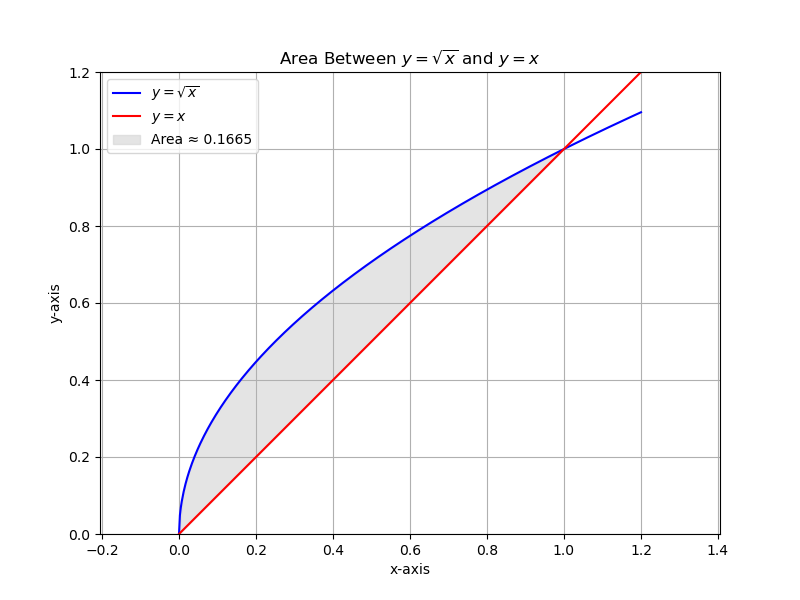
\includegraphics[width=0.8\columnwidth]{../figs/Figure_9.png}
    \caption*{}
    \label{fig:placeholder}
    \end{figure}
\end{frame}

\section{C Code}
\begin{frame}[fragile]{C Code: area\_calculator.c}
\begin{lstlisting}[language=C]
#include <math.h>

double calculate_area(int n) {
    double a = 0.0;
    double b = 1.0;
    double h = (b - a) / n;
    double sum = 0.0;
    
    for (int i = 1; i < n; i++) {
        double x_i = a + i * h;
        sum += sqrt(x_i) - x_i;
    }
    
    double area = h * sum;
    return area;
}
\end{lstlisting}
\end{frame}

\section{Python Code}
\begin{frame}[fragile]{Python Code: main\_caller.py}
\begin{lstlisting}[language=Python]
import ctypes
import os

lib_path = os.path.join(os.getcwd(), 'libarea.so')
area_calculator_lib = ctypes.CDLL(lib_path)

area_calculator_lib.calculate_area.argtypes = [ctypes.c_int]
area_calculator_lib.calculate_area.restype = ctypes.c_double

num_intervals = 100000
area = area_calculator_lib.calculate_area(num_intervals)

print(f"Calculating area using the C library...")
print(f"The calculated area is: {area}")
print(f"The exact area is 1/6 A {1/6}")
\end{lstlisting}
\end{frame}

\begin{frame}[fragile]{Python Code: plotter.py}
\begin{lstlisting}[language=Python]
import numpy as np
import matplotlib.pyplot as plt

x = np.linspace(0, 1.2, 500)
y1 = np.sqrt(x)
y2 = x

fill_x = np.linspace(0, 1, 100)
fill_y1 = np.sqrt(fill_x)
fill_y2 = fill_x

area = np.trapz(fill_y1 - fill_y2, fill_x)

plt.figure(figsize=(8, 6))
plt.plot(x, y1, label=r'$y = \sqrt{x}$', color='blue')
plt.plot(x, y2, label=r'$y = x$', color='red')

plt.fill_between(fill_x, fill_y1, fill_y2, color='lightgray', 
    alpha=0.6, label=f'Area A {area:.4f}')

plt.title('Area Between $y = \sqrt{x}$ and $y = x$')
plt.xlabel('x-axis')
plt.ylabel('y-axis')
plt.legend()
plt.grid(True)
plt.axis('equal')
plt.xlim(0, 1.2)
plt.ylim(0, 1.2)
plt.show()
\end{lstlisting}
\end{frame}

\end{document}